\paragraph{}
Our timeline (Figure~\ref{fig:project_timeline}), named \textit{Muirhead-Scanlon-Yasuna Chart}, depicts a similar setup to the popular Gantt Chart, however, it is not the same. Moreover, it could be considered a derivative of a stripped-down Gantt Chart. Like a Gantt Chart, the $x$-axis expresses time and the $y$-axis lists tasks. In our particular case, time is divided into three sections, one for each WPI term. Under these sections, there exists a subsection for each week of the term. The lowest unit of measurement exists per week of the term, as days from Sunday through Saturday. \TODO Finish.

\begin{figure}[h]
    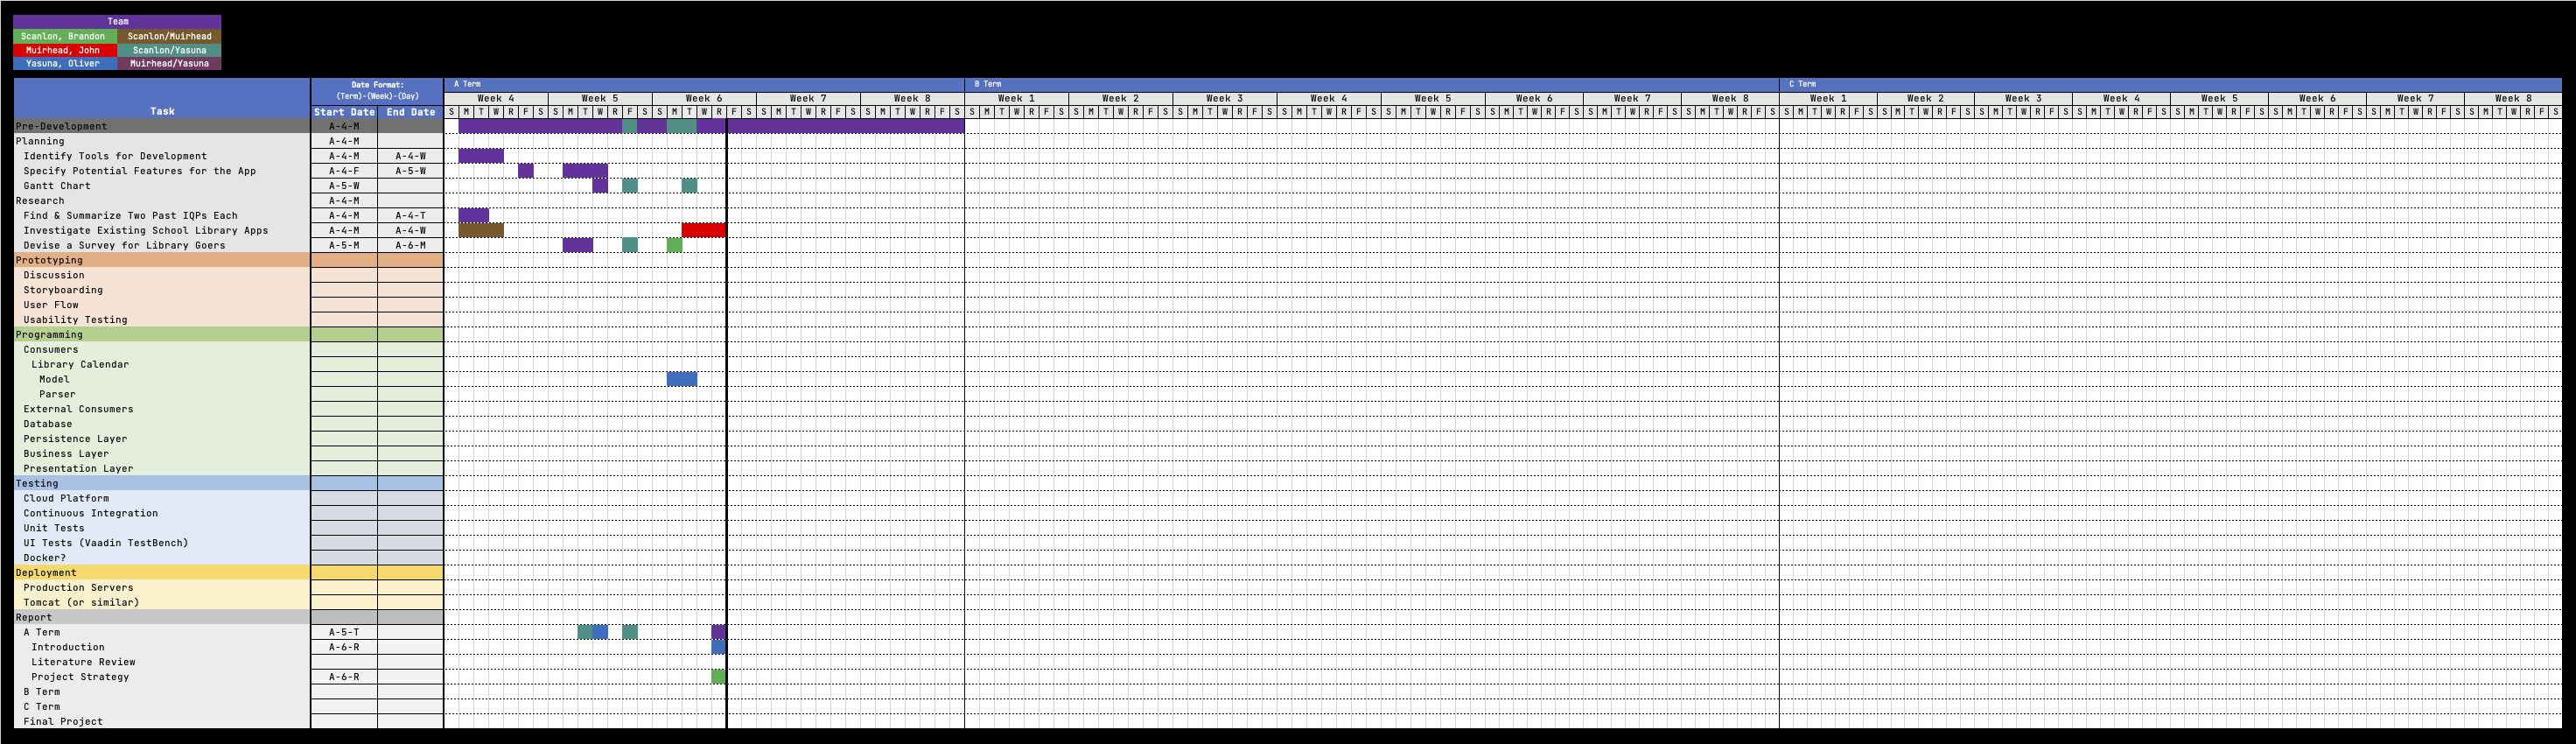
\includegraphics[width = \textwidth, height = \textheight, keepaspectratio]{timeline}
    \caption{Project Timeline}
    \label{fig:project_timeline}
\end{figure}
